%! TEX root = ../main.tex

\section{Solución}
\label{sec:solucion}

\observacion{Ver donde pone la interacción con la cámara}

Se describe la arquitectura propuesta para la realización de una juego serio, se
utiliza la guía básica definida por~\cite{pereira2009design} y descrita
en~\ref{sec:desarrollo}.

Esta sección se enfoca en los aspectos técnicos de la creación del juego serio,
las competencias básicas relacionadas con la educación (segundo paso de la guía
descrita en~\ref{sec:desarrollo}) se define en las
secciones~\ref{sec:glasgow} y~\ref{sec:hemocultivo}.

\subsection{Partes de la simulación}

La simulación se compone de tres elementos principales, entidades (que son
objetos de la vida real), acciones (que son provocadas por las entidades) y
eventos (que son el resultado de una acción). 

Existen otros elementos dentro de la simulación, como la sala y la iluminación,
los mismos son importantes para crear un entorno similar a la realidad y son
estáticos, es decir no interactúan con el usuario más que para limitar la
exploración en el escenario y/o resaltar aspectos relevantes.

\subsubsection{Entidades}

Cualquier objeto o componente en el sistema que requiera la representación
explícita en el modelo\cite{banks2000dm}. Las entidades tienen atributos. Los
atributos son las características de una determinada entidad que son exclusivos
de esa entidad.

Una entidad tiene en todo momento, un estado y una lista de acciones que
puede realizar, esta lista de acciones esta definida por el estado del mismo,
las condiciones en la que se encuentra el entorno y la práctica actual.

La entidad \enquote{Enfermero} es la que es controlada por el usuario, a través
de la interacción con la interfaz gráfica.

\subsubsection{Acciones}

Las entidades se comunican a través de acciones, las cuales pueden tener
diversos orígenes, siempre una entidad inicia una acción. Las acciones provocan
cambios en el ambiente y provocan eventos. Las acciones no solo las
realiza el usuario, sino cualquier entidad.

Como ejemplo, una acción es esterilizar las manos, esta acción provoca un
cambio en el ambiente (las manos ahora son estériles) y fue realizada por la
interacción entre el usuario y la interfaz gráfica.

\subsubsection{Eventos}

Los eventos son ocurrencias instantáneas que cambia el estado de un
sistema\cite{banks2000dm}, cada acción que se realiza provoca una acción, y los
eventos son la mecanismo que tiene una entidad para ser notificada de las
acciones de otras entidades.

\subsubsection{Interacción con el entorno}

El usuario se desenvuelve en un entorno de tres dimensiones, en el cual realiza las
actividades relacionadas a la práctica, se distinguen dos tipos de movimientos
principales que el usuario puede realizar:

\begin{itemize}
    \item \textbf{Alejamiento o acercamiento}: es el acto de acercar o alejar la
        cámara, y por consiguiente al usuario del paciente. Se realiza
        utilizando dos dedos, para realizar un acercamiento, mientras se
        mantiene presionada la pantalla con ambos dedos, se procede a alejar un
        dedo del otro, para realizar un alejamiento, se debe acercar ambos
        dedos.
    \item \textbf{Rotación}: se refiere al movimiento de rotación al rededor de
        un foco, que en ambas escenas es el paciente, para realizara, se utiliza
        un dedo, y se mueve en dedo en cualquier dirección, la cámara, se moverá
        en la dirección contraria.
\end{itemize}

\subsection{Grafo de estados}

La solución tiene varias escenarios, y dentro de cada escenario, existen varias
pantallas que muestran información relevante de acuerdo a la situación de la
simulación, en~\ref{fig:grafo_estados} se observa la interacción entre las
diferentes pantallas y escenarios.

\begin{figure}[H] 
\centering 
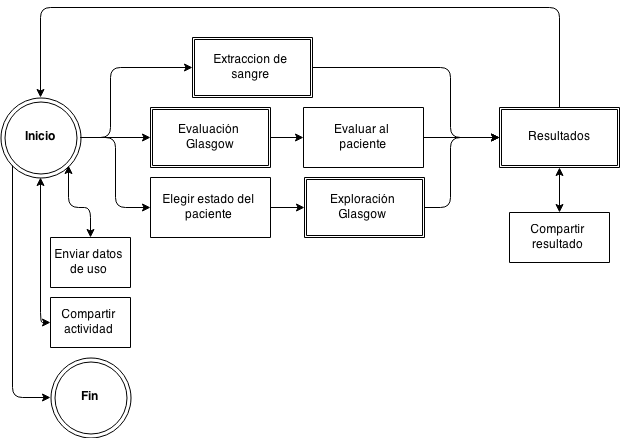
\includegraphics[scale=0.5]{propuesta/grafo_escenas.png}
\caption{Navegación entre escenarios y pantallas. Los escenarios son los
    rectángulos con un borde dos rayas, y las pantallas tienen un borde con una
    sola raya.}
\label{fig:grafo_estados}
\end{figure}

La solución inicia con un escenario denominado \emph{Inicio}, en el cual se
permite al usuario observar los detalles del entorno simulado a la vez que
muestra las opciones que permiten iniciar las diferentes prácticas, compartir
su actividad, enviar los datos de utilización y finalmente salir de la
simulación.

Si el usuario selecciona en el \emph{inicio} la opción \emph{Extracción de
    sangre}, se inicia el escenario denominado \emph{Extracción de sangre}, en
el cual el usuario puede realizar el procedimiento de extracción de sangre, si
el usuario selecciona la opción \emph{Fin}, la simulación termina y se dirige a
el escenario \emph{Pantalla de resultados}.

Al seleccionar la opción \emph{Evaluación Glasgow}, se inicia el escenario
denominado \emph{Glasgow}, donde el usuario debe evaluar a un paciente en el
centro del escenario, si el usuario presiona la opción \emph{Fin} se inicia la
pantalla denominada \emph{Evaluar al paciente}, donde el usuario diagnostica el
estado del paciente, y finalmente al presionar el botón \emph{Fin}, la
simulación finaliza y se inicia el escenario \emph{Pantalla de resultados}.

La opción \emph{Exploración Glasgow} es similar, la diferencia es que antes de
iniciar el escenario \emph{Glasgow}, aparece la pantalla \emph{Elegir estado de
    paciente}, en el cual el usuario selecciona un estado para que el paciente
actué de acuerdo al mismo, luego se inicia la escena \emph{Glasgow} y si el
usuario presiona el botón \emph{Fin}, se inicia el escenario \emph{Pantalla de
    resultados}.

La pantalla de resultados muestra la información acerca de las acciones que
realizo el usuario, proveyendo información a modo de retroalimentación, en esta
pantalla el usuario puede compartir sus resultados por las redes sociales,
reiniciar el escenario y finalmente, poder volver a la \emph{Pantalla de
    inicio}.


\subsection{Inicio}

\subsubsection{Descripción del entorno}

La escena mostrada como pantalla de inicio de la aplicación muestra como fondo la sala de 
un hospital con los elementos típicos de estos lugares, esta es la que se utiliza como 
escenografía principal en los escenas de los procedimientos, haciendo que el usuario entre 
en ambiente. Además de este fondo, se muestras varias opciones en forma de botones que serán 
descriptas a continuación y un mensaje en donde se recomienda al usuario el uso de auriculares.

\subsubsection{Opciones}

Las opciones disponibles en la pantalla de inicio son presentadas en forma de
botones los cuales tienen una breve descripción que identifica la función que
cumplen. 

\todox{Agregar descripción del escenario y si es necesario pantalla donde se
    pone el número}

\begin{itemize}
\item Botón \enquote{Enviar Progreso}: esta función envía toda la información
    acerca de la actividad que el usuario realizo en la aplicación a un servidor
    backend que se encarga de almacenar estos datos.
\item Botón \enquote{Salir de la simulación}: esta función permite salir de la
    aplicación.
\item Botón \enquote{Facebook}: esta función permite al usuario ingresar a su
    cuenta de Facebook.
\item Botón \enquote{Extracción de sangre}: esta función permite ingresar a la
    escena correspondiente al procedimiento de extracción de muestras de sangre
    permitiendo al usuario jugar una nueva partida.
\item Botón \enquote{Explorar Glasgow}: esta función permite ingresar a la
    escena correspondiente al procedimiento para explorar las reacción de un
    paciente con un diagnostico especifico de la escala de Glasgow permitiendo
    al usuario jugar una nueva partida.
\item Botón \enquote{Evaluar Glasgow}: esta función permite ingresar a la escena
    correspondiente al procedimiento para la valoración y diagnostico de la
    escala de Glasgow para un paciente con estado aleatorio permitiendo al
    usuario jugar una nueva partida.
\end{itemize}


\subsection{Extracción de muestras de sangre}

A continuación se detallan cada una de las opciones y formas disponibles de
interactuar con la escena del procedimiento de extracción de muestras de sangre.

\subsubsection{Descripción del entorno}

Al seleccionar el procedimiento de extracción de sangre en la pantalla de inicio 
la aplicación inmediatamente muestra la escena del procedimiento, se muestra una 
sala de hospital igual a la de la pantalla de inicio pero con un paciente en una 
de las camas, a este paciente es a quien se le realizara el procedimiento.

La posición inicial de la cámara se ubica en un ángulo en donde se puedan ver 
bien los brazos del paciente para facilitar al usuario la realización del 
procedimiento.

\todox{Agregar descripción}

\subsubsection{Descripción de la interfaz}

La interfaz principal de este escenario posee dos menús, uno a cada lado de la
pantalla, las opciones son representadas como botones que poseen una imagen
intuitiva\todox{Ver si no hay que agregar esto como hipótesis} que representa la
función que realizan. 

\subsubsection{Entidades}

En la extracción de sangre existen dos entidades principales, el paciente y el
usuario, cada entidad mantiene un estado independiente de la otra entidad.

El paciente es una entidad con estado complejo, el cual es constantemente
modificado por las acciones del usuario, en resumen, la información que contiene
el estado del paciente es:

\begin{itemize}
    \item \textbf{Jeringas}: un paciente puede tener cero o más jeringas en
        cualquier momento, no se limita la cantidad de jeringas que puede
        insertar el usuario.
    \item \textbf{Manos}: almacena el estado de las manos, el paciente reacciona
        ante peticiones del usuario, puede abrir o cerrar cualquier mano en
        cualquier momento.
    \item \textbf{Torniquetes}: es el conjunto de torniquetes que tiene
        actualmente el paciente, notar que los torniquetes pueden ser colocados
        en cualquier parte del brazo, pero existen lugares \enquote{correctos} y
        lugares \enquote{incorrectos}, la diferencia consiste en la distancia a
        los puntos de extracción, estos lugares están predefinidos.
    \item \textbf{Zonas esterilizadas}: son aquellas áreas del cuerpo que el
        usuario esterilizó, no existe un límite para las zonas esterilizadas.
        Una vez que una jeringa es extraída, una zona esterilizada pasa a estar
        contaminada y a la espera de que el usuario la presione.
    \item \textbf{Zonas presionadas}: son aquellas zonas que, una vez
        contaminadas por la extracción de una jeringa, han sido presionadas por
        el usuario.
    \item \textbf{Contaminado}: define si alguna acción realizada por el usuario
        provoco que el paciente se contamine, existen varias cadenas de eventos
        que pueden provocar que esto ocurra:
        \begin{itemize}
            \item Inyección de una jeringa cuando existe otra inyectada.
            \item Inyección en un lugar en lugares inadecuados.
            \item Inyección en un lugar no esterilizado.
            \item Inyección en un brazo cuya mano este abierta.
            \item Inyección fuera del alcance de los torniquetes actuales.
            \item Interacción con el paciente sin que el mismo tenga la mano
                estéril.
        \end{itemize}
        Es importante notar que este estado no es afectado directamente por una
        acción del usuario, sino por la consecuencia de una acción.
\end{itemize}

El \emph{usuario o enfermero} mantiene un estado en todo momento del cual
dependen sus acciones, por ejemplo, si la mano del paciente no esta
esterilizada, cualquier interacción con el paciente provocara que el paciente se
contamine.

\begin{itemize}
    \item \textbf{Manos}: almacena la información acerca de la esterilidad de
        las manos.
    \item \textbf{Guantes, gorro, bata y tapaboca}: almacenan la información
        acerca de los equipamientos que tiene el usuario en un momento dado.
    \item \textbf{Elemento actual}: es el elemento que esta activo en
        cualquier momento, un elemento es una herramienta de la vida real,
        como por ejemplo un torniquete, una gaza.
\end{itemize}

\subsubsection{Acciones}


\paragraph{Comando de voz}

Para representar la interacción del usuario con el paciente usando la voz se
implemento un menú que es activado y mostrado en pantalla cuando el usuario
habla, este menú muestra una seria de ordenes que el usuario le haría al
paciente normalmente hablándole. Las opciones de menú se detalla a continuación:

\begin{itemize}
\item Explicar procedimiento: esta función sirve para detectar si el usuario
    realizo la acción de explicar al paciente acerca del procedimiento. 
\item Abrir la mano izquierda: esta función le indica al paciente que abra su
    mano izquierda, como resultado el paciente realiza esta acción.
\item Cerrar la mano izquierda: esta función le indica al paciente que cierre su
    mano izquierda, como resultado el paciente realiza esta acción.
\item Abrir la mano derecha: esta función le indica al paciente que abra su mano
    derecha, como resultado el paciente realiza esta acción.
\item Cerrar la mano derecha: esta función le indica al paciente que cierre su
    mano derecha, como resultado el paciente realiza esta acción.
\end{itemize}

\paragraph{Opciones}

En este menú se despliegan los botones que representan las opciones de
bioseguridad. Es decir, acciones como lavarse las manos, calzarse guantes,
ponerse gorro, ponerse bata y ponerse tapaboca.

Los elementos de bioseguridad que actualmente tiene puesto el usuario se
representan como se describió anteriormente y se muestran en la parte baja de la
pantalla. Desaparece quitarse que en ese caso se representa al volver a
seleccionar la misma opción.

\paragraph{Elementos}

En este menú se despliegan los botones que representan a lo elementos que se
utilizan para realizar el procedimiento, una vez presionado ese elemento queda
seleccionado. Solo un elemento puede ser seleccionado a la vez. Si el mismo
botón se vuelve a presionar inmediatamente después de haber sido presionado, el
elemento queda de-seleccionado.

%Estas opciones van cambiando el estado del jugador y pueden ser seleccionados
%mas de una opción a la vez además de permitir de-seleccionar una opción
%volviendo a tocar el botón correspondiente. También posee la opción de
%finalizar la partida la cual manda al usuario a la pantalla de resultados.
%% REVISAR ESTO , el comienzo es sobre opciones y el final sobre elementos %%

La herramienta seleccionada actualmente para realizar el procedimiento se se
muestra en la forma descripta anteriormente arriba de la pantalla principal del
procedimiento. Esta imagen representa lo que actualmente tiene en las manos el
jugador. Desaparece al de-seleccionar o terminar de usar la herramienta.

\todox{Agregar colocación}
\todox{Agregar utilización}

\subsubsection{Eventos}
\subsubsection{Motor de reglas}
\subsubsection{Registro de actividad}


\subsection{Valoración de la escala de Glasgow}

\subsubsection{Descripción del escenario}

La interfaz principal de este escenario posee un botón de finalización de
partida al costado con una imagen intuitiva que representa la función que
realiza. Este botón manda al usuario a la pantalla de resultados.

\subsubsection{Entidades}
\subsubsection{Acciones} 
\subsubsection{Eventos} 
\subsubsection{Pantalla de diagnostico}
\subsubsection{Registro de actividad}
\paragraph{Elementos y opciones}


\subsection{Pantalla de resultados}
\subsubsection{Descripción del escenario}
\subsubsection{Retroalimentacion}
\subsubsection{Gamificacion}
\subsubsection{Reinicio}
\subsubsection{Puntuación}
\subsubsection{Tiempo utilizado}
\subsubsection{Facebook 2}

\subsection{Partes de la simulación}
    \subsubsection{Entidades}
    \subsubsection{Eventos}
    \subsubsection{Acciones}
    \subsubsection{Interacción con la cámara}

\subsection{Grafo del desarrollo}
% podemos poner acá un gráfico mas o menos así (ver graphviz)
%           /---> Hemocultivo --\
%          /                     \              /-> Reiniciar
%  Inicio ------> Glasgow 1 -------> Resultados --> Inicio
%         \ \                    /              \-> Facebook 2
%          \ \--> Glasgow 2 ----/
%           \---> Salir 
%            \--> Facebook 1
%             \-> Enviar resultados

\subsection{Pantalla de inicio}
    \subsubsection{Descripción del escenario}
    \subsubsection{Enviar datos}
    \subsubsection{Glasgow}
    \subsubsection{Extracción de sangre}
    \subsubsection{Facebook 1}

\subsection{Extracción de sangre}
    \subsubsection{Descripción del escenario}
    \subsubsection{Descripción de la interfaz}
    \subsubsection{Entidades} % definimos cuales son las entidades
        %\subsubsubsection{Estado del enfermero}
        %\subsubsubsection{Objeto seleccionado}
    \subsubsection{Acciones} % definimos cuales son las acciones de esas entidades
        %\subsubsubsection{Comandos de voz}
        %\subsubsubsection{Opciones} %bata,mano,guante,y eso
        %\subsubsubsection{Elementos}
            %\subsubsubsubsection{Colocación}
            %\subsubsubsubsection{Utilización}
    \subsubsection{Eventos} % definimos cuales son los eventos que se lanzan en este proceso
    \subsubsection{Motor de reglas} % se define como funciona el motor de reglas acá
    \subsubsection{Registro de actividad} % se define como se registra las acciones del usuario (cuales)


\subsection{Glasgow 1 y 2}
    \subsubsection{Descripción del escenario}
    \subsubsection{Entidades} % definimos cuales son las entidades
        %\subsubsubsection{Reacciones del paciente}
    \subsubsection{Acciones} % definimos cuales son las acciones de esas entidades
        %\subsubsubsection{Acciones sobre el paciente}
        %\subsubsubsection{Comandos de voz}
    \subsubsection{Eventos} % definimos cuales son los eventos que se lanzan en este proceso
    \subsubsection{Pantalla de diagnostico}
    \subsubsection{Registro de actividad} % se define como se registra las acciones del usuario (cuales)
    
\subsection{Pantalla de resultados}
    \subsubsection{Descripción del escenario}
    \subsubsection{Retroalimentacion}
    \subsubsection{Gamificacion}
    \subsubsection{Reinicio}
    \subsubsection{Puntuación}
    \subsubsection{Tiempo utilizado}
    \subsubsection{Facebook 2}
